\subsection{External Interface Requirements}
\subsubsection{System Interfaces}
The NavUp systems’ interfaces include locating and retrieving site information (building names, addresses, etc.) based on the information retrieved from the Navigation module. The site information will be used for gathering and maintaining any information of interest with regard to the “searched” location. The acquired information about the location will be stored and pushed as a notification to the users’ interface where users can view and read it.

\subsubsection{User Interfaces}
The system will allow users to find locations, so the route guidelines to the destination will be displayed on the users’ screen interface, route guidelines include a pin-point indicating users’ current positon, colored route path to the destination, and the pin-point indicating the destination. So, once the information of interest with regard to the location has been acquired, the information will be sent to the user as a notification, and the notification may be in a form of SMS, E-mail, or a push notification. The user will have an option to alter how the notifications are received, that is, either as an E-mail, push notification or an SMS.

\subsubsection{Hardware Interfaces}
The Wi-Fi routers and mobile phones are the only primary hardware interfaces that may be required for the “points of interest” module. Mobile phones will be used for all the user interfaces and the functionality of the NavUp system and the Wi-Fi access points as a reference for detecting locations both indoors and outdoors.

\subsubsection{Software Interfaces}
The NavUp will primarily run on mobile phones. Therefore, for compatibility requirements, the NavUp system should be hybrid, that is, it has to be compatible across most, if not all ranges of mobile smart phones and mobile operating systems, that is either Android OS, iOS, or Microsoft Windows. The system can also be web-based.

\subsubsection{Communication Interfaces}
The system will frequently communicate with the campus map database, servers and the mobiles’ GPS to get locations and directions through Wi-Fi networking. Any acquired information of interest with regard to the desired location may be retrieved from the database through servers. The systems’ communication interface may also include web services.
		
\subsection{Performance Requirements}
\subsubsection{Track creation/ Route update}
The NavUp system should also keep track of the user's current locationso to update the route displayed on the user's screen interface, however the system should not necessarily update the route every after 1 second, the route update can be in an interval of 7 seconds per update.

\subsubsection{User login response time}
The users will be required to login, provided that the user has entered correct credentials, the NavUp system should take no longer
than 6 seconds to provide full system access to the user. However, this may be dependent on the internet connection bandwith.
	
\subsubsection{Positional accuracy}
Accuracy is one of the vital performance required for the system. The NavUp system should be accurate enough to get the user’s current position, if for example the user is in the building (indoor) with multiple floors, the system should not necessarily determine the exact venue, but it should be in range and	in real time.\\\\ 
The system should have a good ranging accuracy. The accuracy of the system is defined as the solution error, and the accuracy of the system should conform to position range and the PVT (Position, Velocity and Time). This will be useful in terms of “points of interest” where accuracy is very important when determining locations.

\subsubsection{Proximity of notifications}
The user will recieve any information of interest for the locations he/she visits, the amount of time it takes to recieve the notification shouldn't be long, this is to say, the system should be responsive enough to an extent that when the user gets to the desired location, it takes no longer than 25 seconds to recieve the notification.
  	
 \subsection{Design Canstraints}
 Getting the current location will be difficult using WiFi because it is hard to triangulate the position of one device due to the face that the WiFi signal will not give you an accurate representation of where the device is. At best the current location might vary by 10m to 15m depending on the objects it had to pass though e.g. wall or roof. If the user cannot get WiFi signal it will be hard for the user to get the current location because then it will be using the users data and the user might be reluctant to allow that. 	
  	
\subsection{Software System Attributes}
    \subsubsection{Accuracy}
        The data of the points of interest module needs to be accurate. The saved location of a point of interest needs to be accurate for the navigation module to navigate the user to the point of interest. The information about the point of interest also needs to be accurate to avoid misinformation.
    \subsubsection{Reusability}
        The points of interest module should be able to support multiple different types of locations like lecture halls, museums, restaurants, etc. The module should be able to add new types of locations without the need for extending the app.
    \subsubsection{Usability}
        A point of interest should be easy to find on the campus map as well as being searchable in the database. The icons on the map should also be relevant and intuitive for the different types of points of interest. The location information should also be easy to find once the user has accessed the point of interest. 
    \subsubsection{Maintainability}
        The points of interest needs to be maintained. When there are new points of interests they need to be added to the system. If a point of interest has new information it needs to be updated in the system.

\subsection{Class Diagram}
\begin{figure}[H]
	\centering
	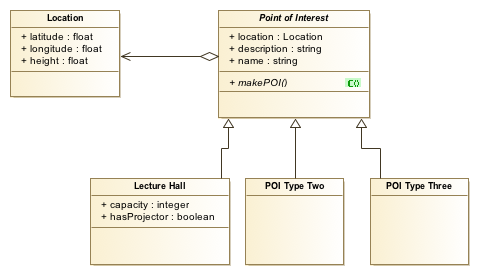
\includegraphics[scale=0.54]{POI/poi_class_diagram.png}
	\caption{POI Class Diagram}
	\label{fig:POI_Class_Diagram}
\end{figure}

\subsection{Design Patterns Used}
    \paragraph{Factory Method}
    The points of interest module needs to be able to implement different types of points of interest. The factory method defines an interface for creating an object, but lets subclasses decide which class to instantiate. Factory Method lets a class defer instantiation to subclasses. Because instantiation is deferred to subclasses it is possible to have many different types of points of interest classes which inherit from the abstract Point of Interest class.
 
 \subsection{Activity Diagram}
\begin{figure}[H]
	\centering
	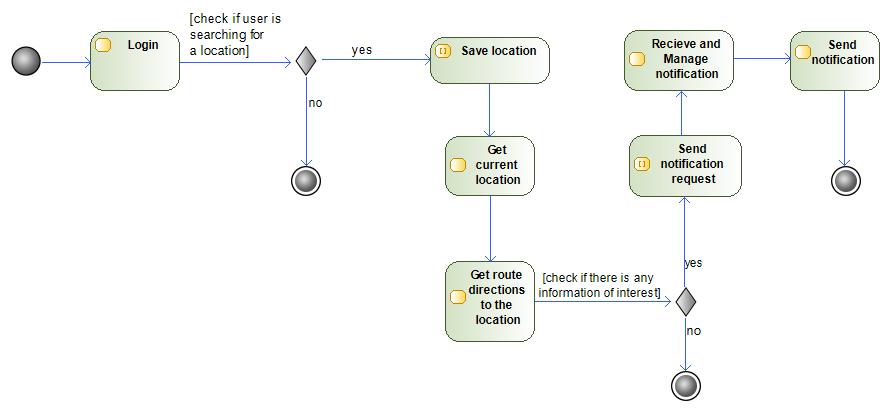
\includegraphics[scale=0.54]{POI/poi_activity_diagram.png}
	\caption{POI Activity Diagram}
	\label{fig:POI_Activity_Diagram}
\end{figure}

 \subsection{Sequence Diagram}
\begin{figure}[H]
	\centering
	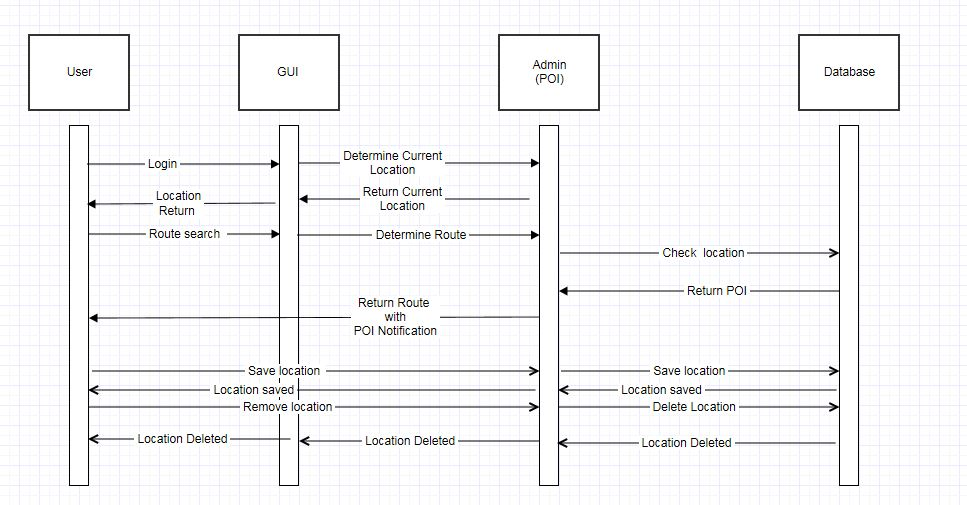
\includegraphics[scale=0.54]{POI/poi_sequence_diagram.JPG}
	\caption{POI Sequenc Diagram}
	\label{fig:POI_Sequence_Diagram}
\end{figure}

 \subsection{State Diagram}
\begin{figure}[H]
	\centering
	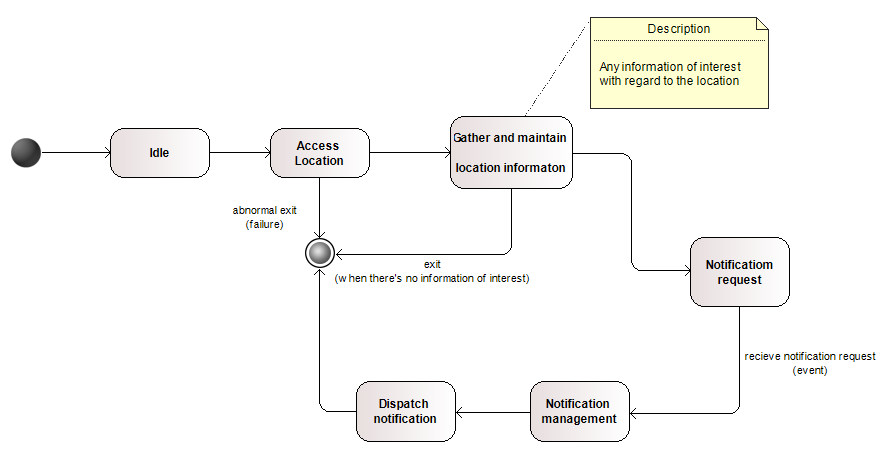
\includegraphics[scale=0.54]{POI/poi_state_diagram.png}
	\caption{POI State Diagram}
	\label{fig:POI_State_Diagram}
\end{figure}
		
 \subsection{Use Case Diagram}
\begin{figure}[H]
	\centering
	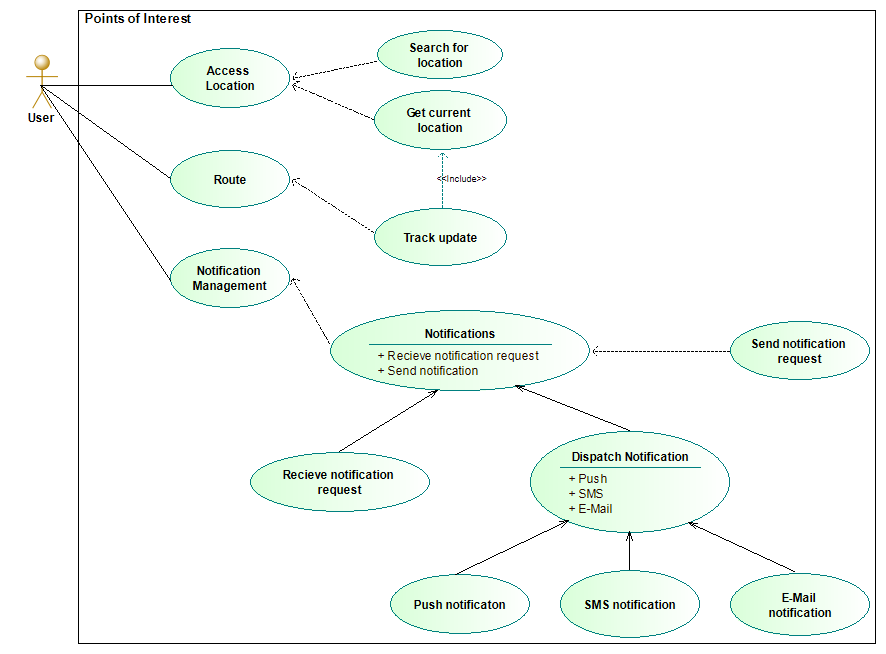
\includegraphics[scale=0.54]{POI/poi_use_case_diagram.png}
	\caption{POI Use Case Diagram}
	\label{fig:POI_Use_Case_Diagram}
\end{figure}
